\section{问题二:不确定性环境下的鲁棒优化模型}

面对未来市场与生产环境中的不确定性,原有的确定性优化模型已不再适用。问题二的核心要求,是从寻求单一情景下的最优解,转变为在众多可能的未来情景中,制定一个能够抵御风险、综合表现稳健的种植策略。为此,本章建立了一个鲁棒优化框架,如图\ref{fig:robustness_framework}所示。该框架的目标是在所有预设的不确定性扰动下,寻求一个能够保障最低利润水平的种植方案。


\begin{figure}[H]
	\centering
	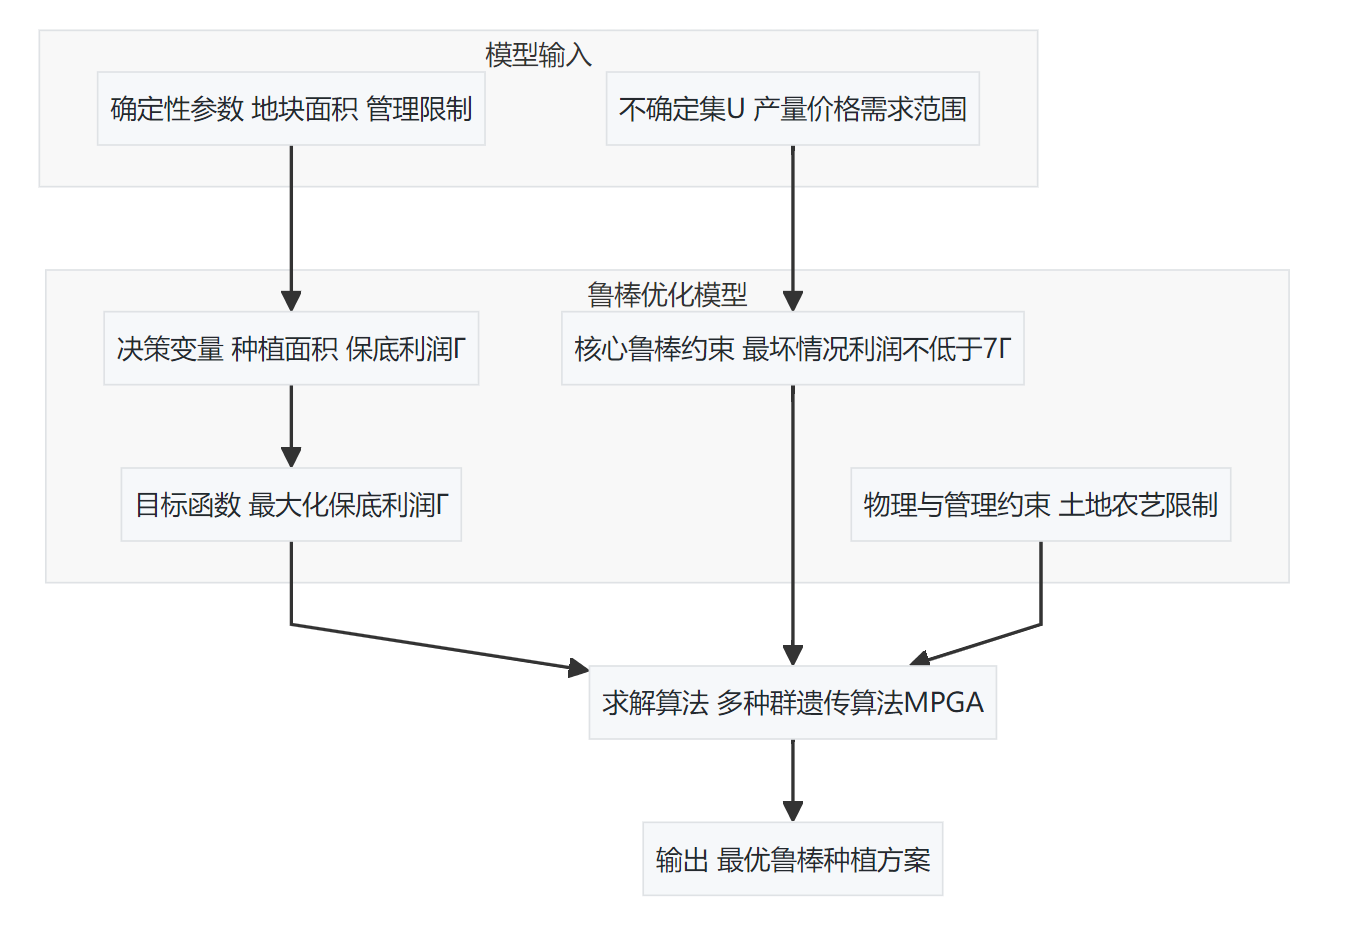
\includegraphics[width=0.9\textwidth]{figs/4问题二/问题二框架.png}
	\caption{鲁棒优化框架}
	\label{fig:robustness_framework}
\end{figure}


\subsection{模型构建}
我们选择以问题一中的情景二作为市场基础反应机制,即产量超出预期的部分按正常价格的50\%销售。我们认为这种设定比完全滞销更能反映现实市场的供需调节能力,并在此基础上构建鲁棒优化模型。

\subsubsection{参数与不确定集}
模型参数分为确定性与不确定性两类。地块面积 $A_i$、地块内作物种类上限 $p$、作物跨地块类型上限 $q$ 等属于确定性参数。另一部分关键参数则是不确定的,它们在一个预设的区间(即不确定集 $U$)内波动。
\begin{itemize}
	\item \textbf{亩产量 ($yield_{jy}$)}: 受气候等因素影响,年亩产量在上一年度基准值的90\%至110\%之间波动。
	\item \textbf{预期销售量 ($sale_{jy}$)}: 小麦和玉米的需求呈增长趋势,年增长率介于5\%至10\%;其他作物的年需求量则在上一年度基准值的95\%至105\%之间变动。
	\item \textbf{种植成本 ($C_{jy}$)}: 成本被视为确定性增长,每年递增5\%。
	\item \textbf{销售价格 ($P_{jy}$)}: 粮食类价格稳定;蔬菜类价格每年增长5\%;羊肚菌价格每年下降5\%;其他食用菌价格年下降率介于1\%至5\%之间。
\end{itemize}

\subsubsection{决策变量与目标函数}
本模型的核心决策变量是在年份 $y$ 的第 $k$ 季,于地块 $i$ 上种植作物 $j$ 的面积 $a_{ijky}$,以及相应的二进制变量 $x_{ijky}$。此外,引入辅助变量 $normal_{jy}$ 和 $over_{jy}$ 分别表示正常销售和降价销售的产量。

区别于传统优化模型,本模型引入了一个关键的决策变量 $\Gamma$,它代表七年规划期内的年度平均保底利润。整个优化模型的目标,是最大化这个在最坏情况下依然能够实现的年度平均保底利润 $\Gamma$。
\begin{equation}
	\text{Maximize} \quad \Gamma \label{eq:objective}
\end{equation}

\subsubsection{约束条件}
为实现上述目标,模型建立在一系列约束之上,其中核心是鲁棒约束。
\begin{enumerate}
	\item \textbf{核心鲁棒约束}: 该约束是鲁棒优化的关键。它要求在不确定集 $U$ 内的任何一种场景组合下,七年的累计总利润都不得低于由保底利润 $\Gamma$ 定义的总目标值。
	      \begin{equation}
		      \sum_{y \in Y} \text{Profit}_y \ge 7 \cdot \Gamma, \quad \forall (yield, sale, C, P) \in U \label{eq:robust_core}
	      \end{equation}
	      其中,年度利润 $\text{Profit}_y$ 的计算方式为:
	      \begin{equation}
		      \text{Profit}_y = \sum_{j \in J} (normal_{jy} \cdot P_{jy} + over_{jy} \cdot 0.5 \cdot P_{jy}) - \sum_{i,j,k} a_{ijky} \cdot C_{jy} \label{eq:profit_calc}
	      \end{equation}

	\item \textbf{产量与销售关联约束}: 作物的总产量等于正常销售量与降价销售量之和,此关系在所有可能的亩产量场景下均须成立。
	      \begin{equation}
		      \sum_{i,k} a_{ijky} \cdot yield_{jy} = normal_{jy} + over_{jy}, \quad \forall j, y, \forall yield_{jy} \in U_{yield} \label{eq:yield_balance}
	      \end{equation}

	\item \textbf{鲁棒化的正常销售上限约束}: 为确保方案的可行性,正常价格销售的产量部分不应超过在任何需求波动下都能实现的最低预期销售量。
	      \begin{equation}
		      normal_{jy} \le \underline{sale}_{jy}, \quad \forall j,y \label{eq:sale_limit_robust}
	      \end{equation}
	      其中 $\underline{sale}_{jy}$ 是作物 $j$ 在年份 $y$ 的预期销售量下限。

	\item \textbf{物理与管理约束}: 此部分约束与问题一基本一致,包括决策变量关联、土地适宜性、地块面积限制、重茬约束、豆类轮作要求 以及作物分散性限制。
\end{enumerate}

\subsection{模型求解:多种群遗传算法}
为求解上述随机优化问题,我们采用了多种群遗传算法(Multi-Population Genetic Algorithm, MPGA)。标准的遗传算法在处理复杂解空间时,可能因种群多样性过早丧失而收敛到局部最优解。多种群遗传算法通过将整个种群划分为若干个并行的、相对独立的子种群来应对这一挑战。每个子种群独立进行选择、交叉和变异等进化操作,这种并行搜索机制有助于维持整个种群的探索能力。具体机制如图\ref{fig:transfer_operator}所示。

\begin{figure}[H]
	\centering
	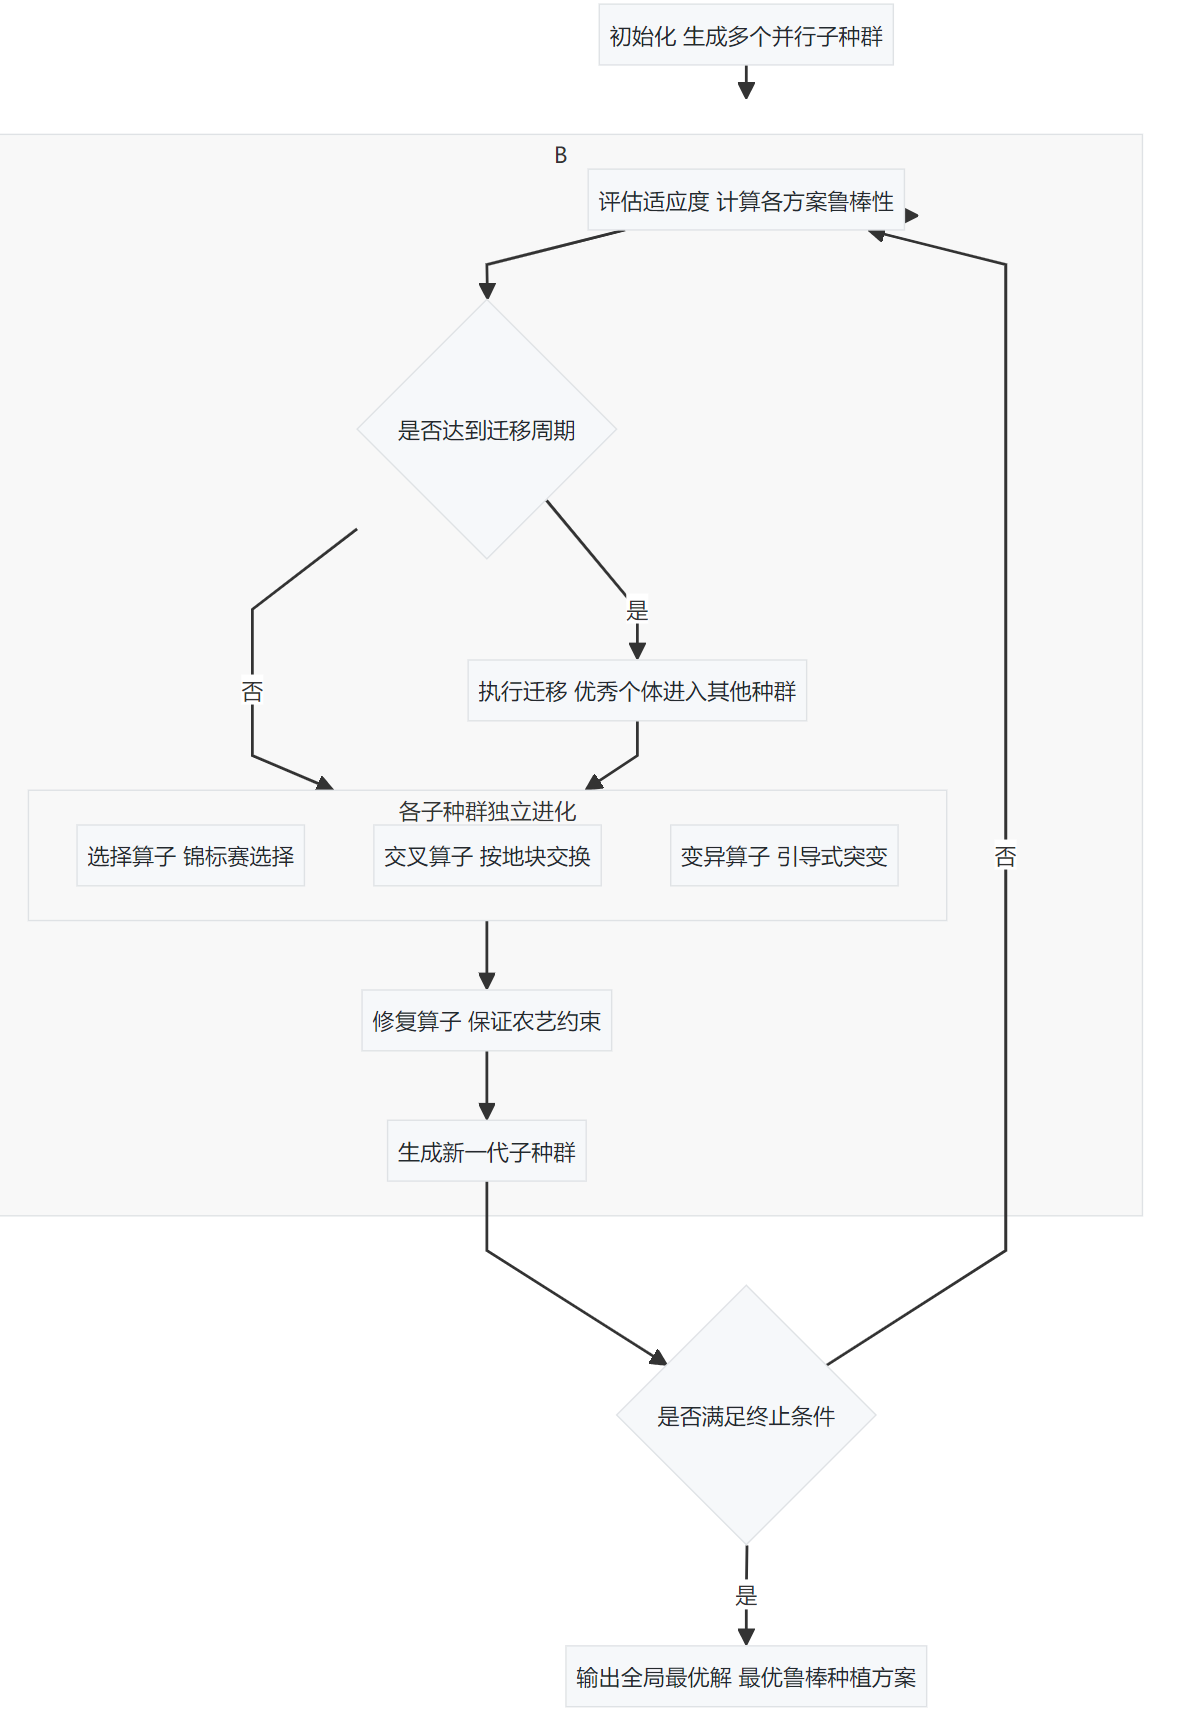
\includegraphics[width=0.7\textwidth]{figs/4问题二/多种群遗传算法.png}
	\caption{遗传算法迁移算子}
	\label{fig:transfer_operator}
\end{figure}



为促进子种群之间的信息交流,避免各个子种群陷入孤立的局部最优点,算法还引入了迁移算子。该算子以预设的代数间隔,将优势子种群中的最优个体迁移到其他子种群中,以替换其中的较差个体。这种机制使得各个子种群的优良基因得以在整个大种群中扩散,从而引导算法向全局更优的区域探索。图\ref{fig:convergence_comparison}展示了多种群遗传算法相对于标准遗传算法在收敛性能上的优势。标准算法可能在早期就陷入停滞,而多种群算法则能够持续优化,最终收敛到质量更高的解。

\begin{figure}[H]
    \centering
    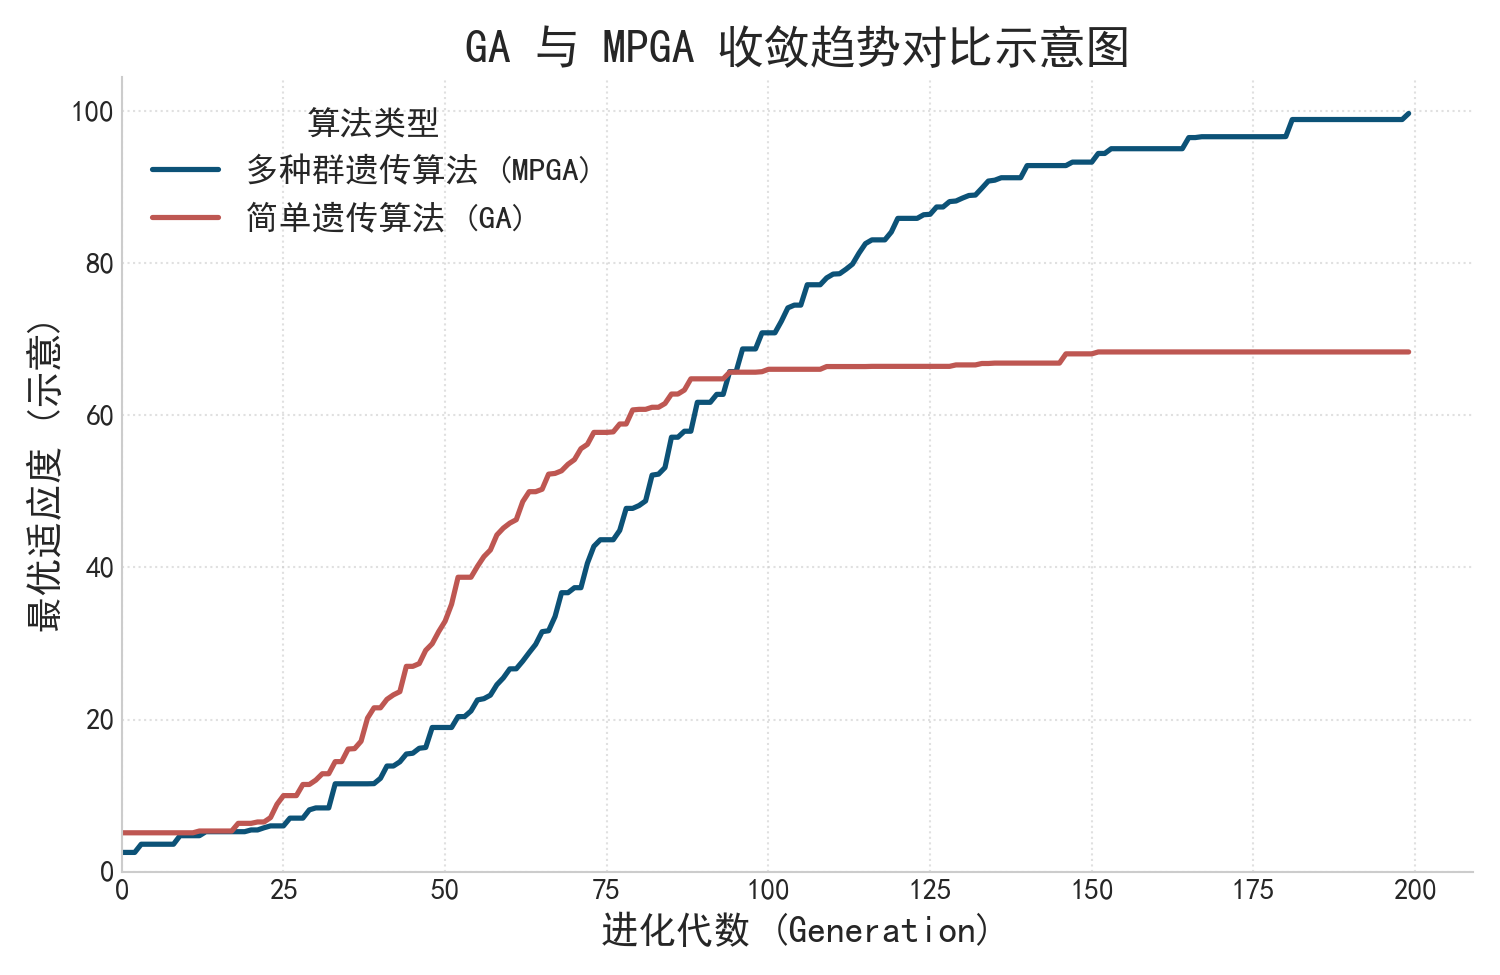
\includegraphics[width=0.7\textwidth]{figs/4问题二/遗传算法收敛对比图.png}

    \caption{多种群遗传算法与标准遗传算法收敛过程对比}
    \label{fig:convergence_comparison}
\end{figure}

算法的实现细节中,解决方案的编码、遗传算子与问题一保持一致。此外,为保证所有生成的解始终满足农艺要求,算法在每次交叉和变异操作后,均调用修复函数来处理重茬与豆类轮作这两项硬性约束。

\subsection{结果与分析}

\subsubsection{多方案评估与最优决策}
由于风险偏好系数$a$的取值直接影响最终方案的风险收益特征,我们选取了$a \in \{0.1, 0.3, 0.5, 0.7, 0.9\}$五个代表性的水平,并对每个水平独立运行MPGA优化,得到了一系列位于有效前沿上的候选方案。表\ref{tab:sensitivity_results}汇总了这些方案在期望利润、最低利润、风险以及夏普比率四个核心指标上的表现。

\begin{table}[H]
    \centering
    \caption{不同风险偏好下的方案性能指标}
    \label{tab:sensitivity_results}
    \begin{tabular}{@{}lcccc@{}}
        \toprule
        风险系数 $a$ & 期望利润 (百万元) & 最低利润 (百万元) & 风险 (标准差, 百万元) & 夏普比率 \\
        \midrule
        0.10 & 41.50 & 40.35 & 0.77 & 53.90 \\
        0.30 & 42.75 & 41.50 & 0.83 & 51.51 \\
        0.50 & 43.60 & 42.40 & 0.80 & 54.50 \\
        \textbf{0.70} & \textbf{44.15} & \textbf{43.10} & \textbf{0.70} & \textbf{63.07} \\
        0.90 & 44.80 & 43.50 & 0.87 & 51.49 \\
        \bottomrule
    \end{tabular}
\end{table}

数据显示,$a=0.7$对应的方案在各项指标中取得了最佳的综合平衡。该方案的夏普比率达到63.07,在所有候选中最高,表明其风险调整后的收益效率最优。同时,该方案的风险水平(标准差0.70百万元)为所有候选中最低,而其期望利润(44.15百万元)和最低利润(43.10百万元)均处于高位。图\ref{fig:sensitivity_combo}也直观展示了各方案在不同指标下的表现。基于此综合评估,我们将$a=0.7$的方案确定为问题二的最终推荐方案。

\begin{figure}[H]
    \centering
    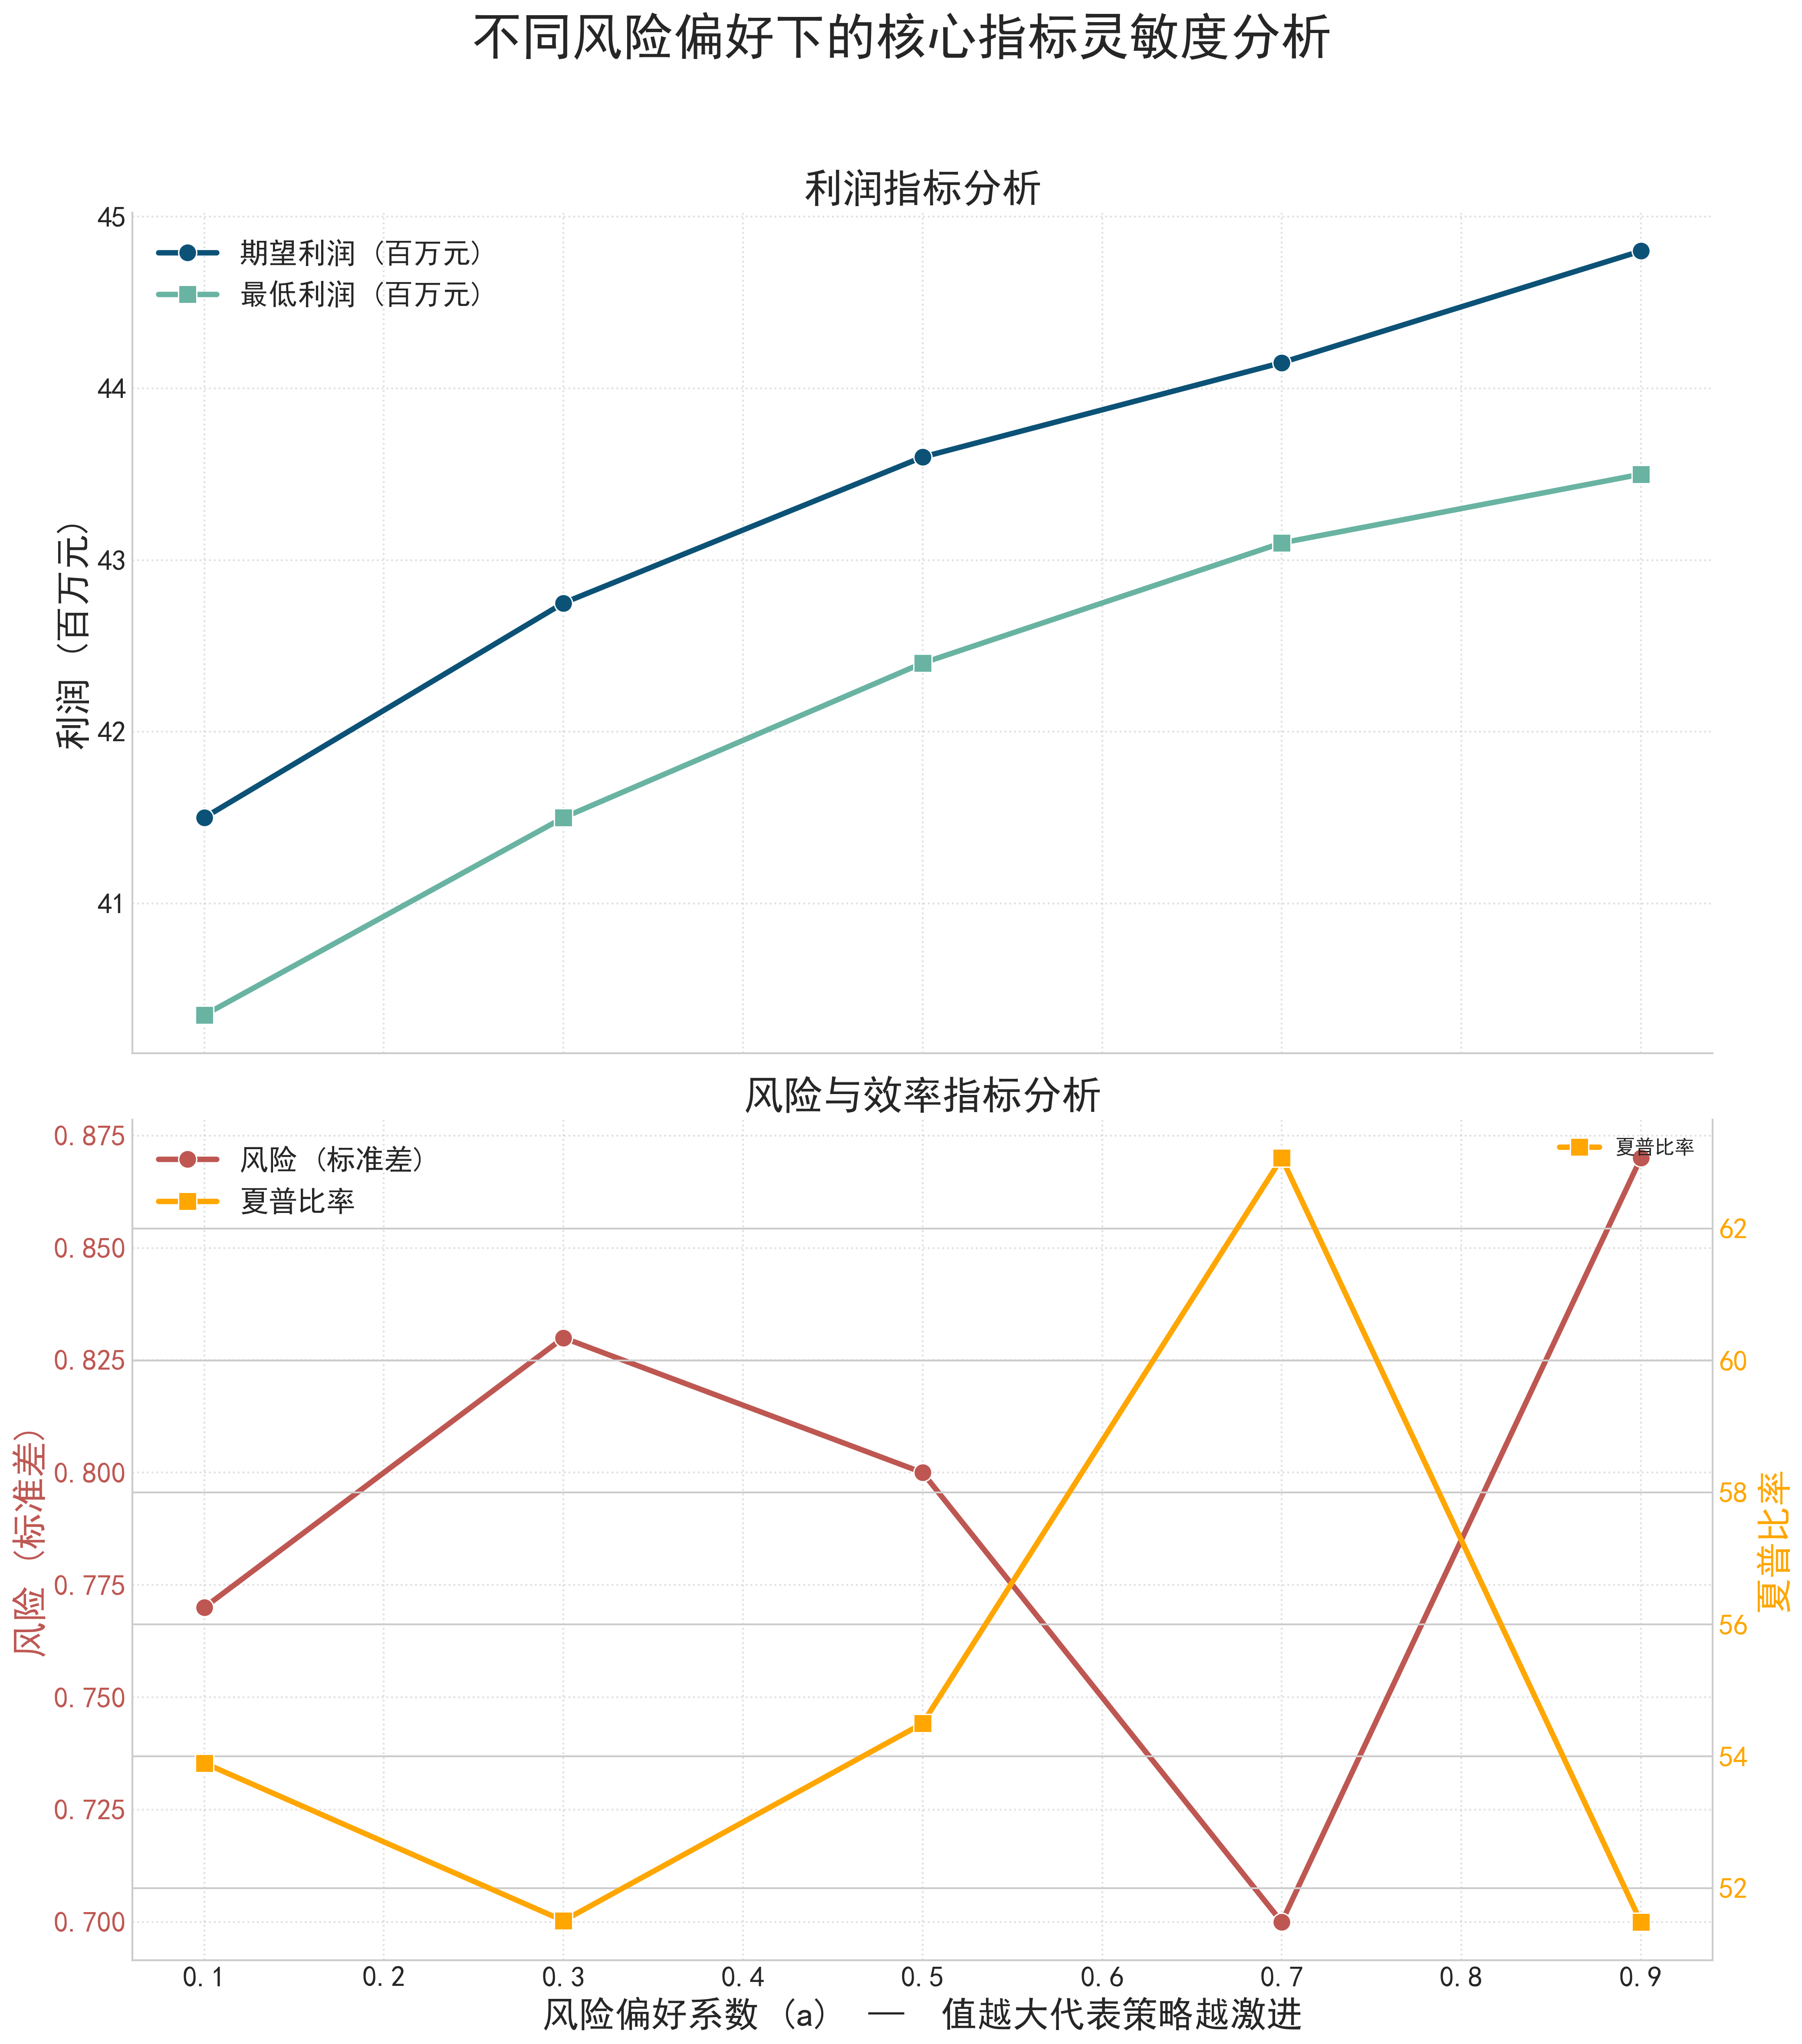
\includegraphics[width=\textwidth]{figs/4问题二/多指标灵敏度分析组合图.png}
    \caption{多指标灵敏度分析组合图}
    \label{fig:sensitivity_combo}
\end{figure}

\subsubsection{最优方案鲁棒性验证}
为验证本章所提出鲁棒优化方案的有效性,我们将其与问题一(情景二)中得到的确定性优化方案进行了对比。两个方案在10000个相同的随机未来情景下进行模拟测试,其最终利润的统计分布如图\ref{fig:robustness_dist}所示。

\begin{figure}[H]
    \centering
    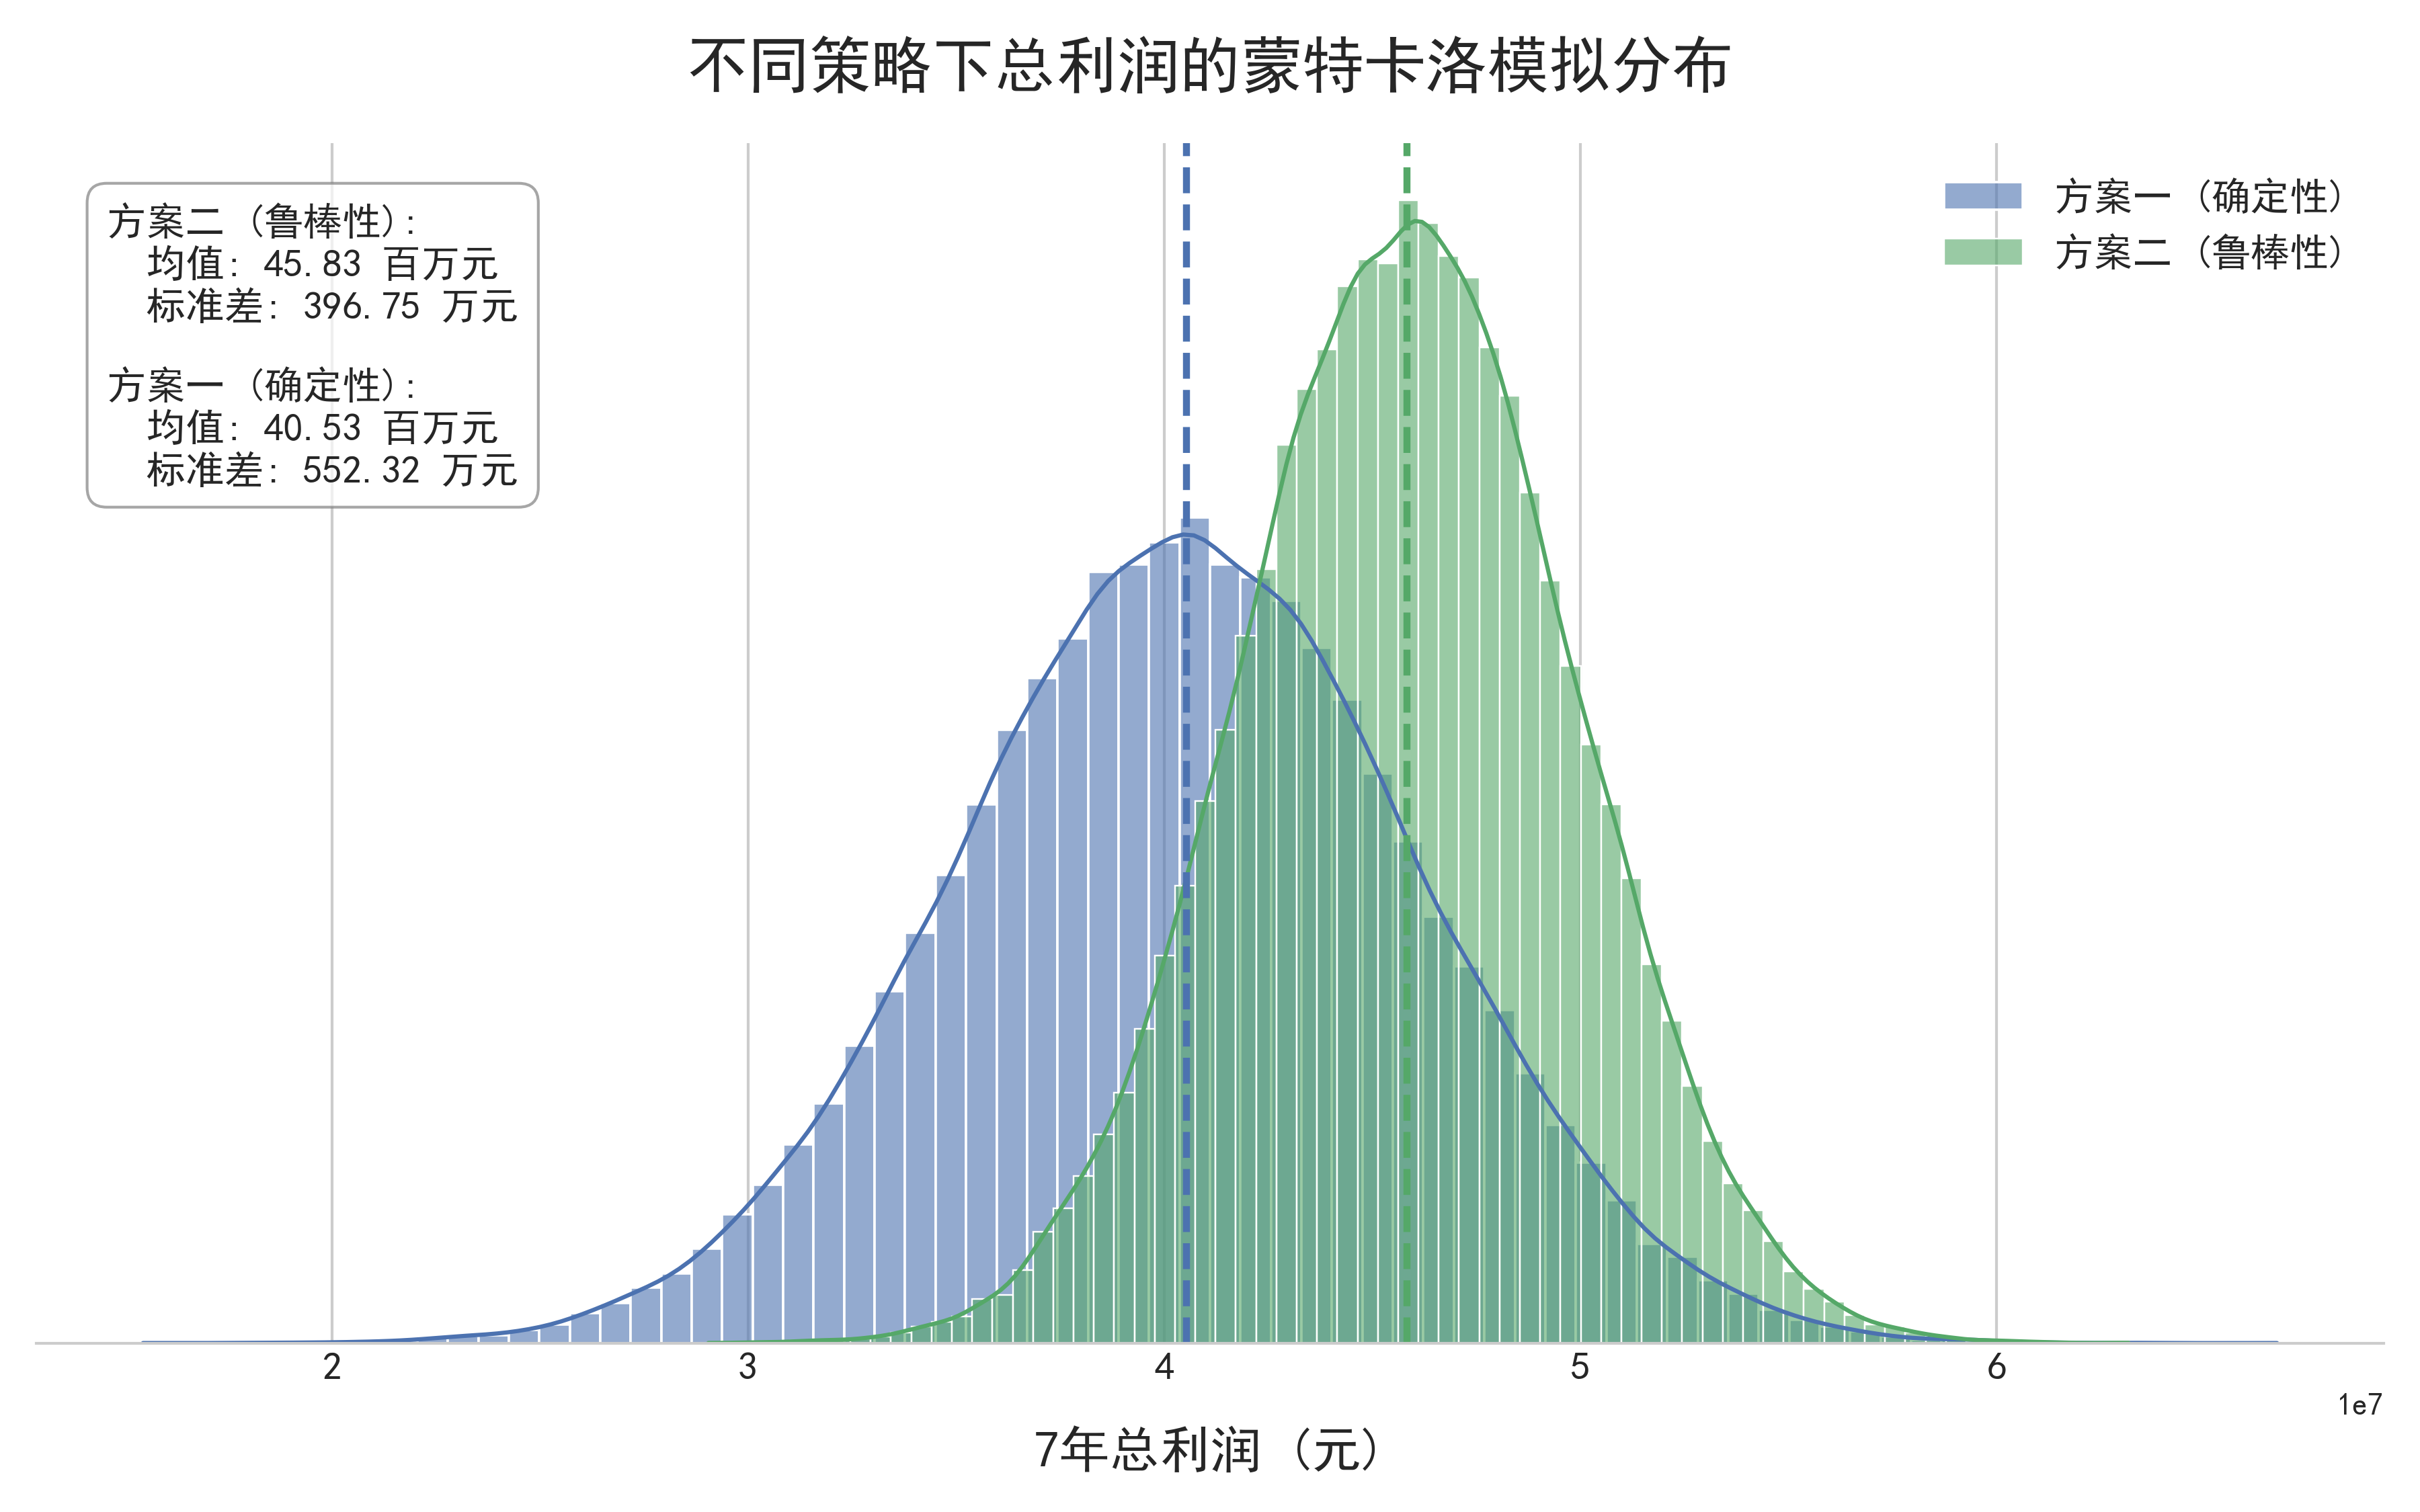
\includegraphics[width=\textwidth]{figs/4问题二/鲁棒性蒙德卡诺模拟分布图.png}
    \caption{鲁棒方案与确定性方案的利润分布对比}
    \label{fig:robustness_dist}
\end{figure}

模拟结果表明,问题一的确定性方案在不确定环境下的期望利润为40.53百万元,利润标准差为5.52百万元。相比之下,本章得到的鲁棒优化方案,其期望利润提升至45.83百万元,而利润标准差则降低至3.97百万元。这一结果有力地证明,通过在优化过程中系统性地考虑不确定性,所得到的鲁棒方案不仅显著降低了未来收益的波动风险,同时也通过把握市场增长趋势,获得了更高的期望收益,其综合性能远优于确定性模型下的最优解。

